\documentclass[review]{elsarticle}

\usepackage{enumitem}
\usepackage{hyperref}
\usepackage{xcolor}
\hypersetup{
    colorlinks,
    linkcolor={red!50!black},
    citecolor={blue!50!black},
    urlcolor={blue!80!black},
    pdfborder={0 0 0}
}
\usepackage{multirow}
\usepackage{pgfplots}
\usepackage{float}
\usepackage{amssymb}
\usepackage{cleveref}
\usepackage[english]{babel}
\usepackage[utf8]{inputenc}
\usepackage[T1]{fontenc}
% \usepackage{changepage}
\usepackage{longtable}
\usepackage{tabularx}
% \usepackage[showframe=true]{geometry}
%
\newcommand{\textttt}[1] {\texttt{\footnotesize#1}}
\newcommand{\h} {\hphantom ~ }
% \newcommand{\textttt}[1] {\mbox{\texttt{\footnotesize#1}}}
% \newcommand{\textttt}[1] {
% \begin{verbatim} #1 \end{verbatim}
% }
\pgfplotsset{compat=1.5}
\pgfplotsset
{
	width=0.5\textwidth,
	x tick label style={/pgf/number format/1000 sep=},
  enlarge x limits = 0.0,
  ymajorgrids=true,
	major tick style={draw=none},
  ymin = 0.0,
	every axis/.append style={
		every x tick label/.append style={font=\tiny},
    every y tick label/.append style={font=\tiny},
    every axis label/.append style={font=\small},
    height=37mm,
    width=37mm,
    title style={at={(0.5,0.90)}, font=\normalfont},
    xticklabel style={yshift=4pt}
	}
}

%% `Elsevier LaTeX' style
\bibliographystyle{elsarticle-num}
%
\makeatletter
\def\ps@pprintTitle{%
    \let\@oddhead\@empty
    \let\@evenhead\@empty
    \def\@oddfoot{}%
\let\@evenfoot\@oddfoot}
\makeatother
\begin{document}
%
\begin{frontmatter}
%
\title{A Linked Open Social Database for Scientific Benchmarking}
%
\author[pwr]{Renato Fabbri\corref{corresponding}\fnref{kio-url}}
\ead{fabbri@usp.br}
%
\author[pwr]{Osvaldo Novais de Oliveira Junior\fnref{kio-url}}
\ead{chu@ifsc.usp.br}
%
\cortext[corresponding]{Corresponding author}
\address[pwr]{S\~ao Carlos Institute of Physics, S\~ao Paulo
University, Brazil}
%
\fntext[kio-url]{\textit{URL:} \url{http://www.ifsc.usp.br/}}
%
\begin{abstract}
The fields of social network analysis and complex networks
are widely researched.
Recently, a myriad of results have been reported which are based in
diverse datasets most often not accessible to researchers other than the publishing authors.
This work exposes an open database with diverse provenance and oriented
to furnish the scientific community with a friendly and common repertoire.
Current data was obtained from Facebook, Twitter, IRC, Email and the
detached instances of ParticipaBR, AA and Cidade Democr\'atica.
These were represented as linked data to homonenize access,
conform to current best practices and ease analyzes which integrate third
party and provided instances.
This document presents an outline and overall statistics of the given
database which should favor subsequent work.
\end{abstract}
%
\begin{keyword}
Big Data, Data Mining, Benchmark Data, Facebook, Twitter, IRC, Email,
Complex Networks, Text Mining
%Hierarchy of Clusters \sep HoC \sep Benchmark Dataset \sep Benchmark Data Generator \sep Artificial Data \sep Cluster Analysis \sep Tree Structured Stick Breaking Process \sep TSSB \sep ...
\end{keyword}

\end{frontmatter}

\section{Introduction}


% In recent years, the web of linked data~\cite{lee1} has attracted wide attention in
% both research and application realms.
Open machine-readable contents and tools are desired
in performing knowledge discovery in social data.
% there is a lack of datasets for benchmarking results,
However, there is a lack of open datasets for benchmarking results,
specially associated to the complex networks field,
yielding diverse results from poorly related sources.

The enormity of the digital data propels a rapid development of analysis methods
from different perspectives.
Even so, the used datasets in the literature differ within the scope of each research with
scarce and historical exceptions such as the
karate club dataset~\cite{newmanBook}.
Beyond that, the available linked data is not 
stable or rigorous enough to be
a public reference on statistical physics and social networks research.
 
This work presents a framework that provides machine-readable contents with a
database on social networks.
This has been made by linkng social data into an open database with diverse
provenance, including Facebook, Twitter, IRC, Email and detached
instances.
Such data is proposed as a common repertoire for scientific
research involving networks and textual content and may be extended.

% \subsection{Benchmarking in the analysis of complexity}

\section{Materials}\label{materials}
Data was gathered from:
\begin{itemize}
    \item public APIs (Twitter, Email);
    \item public logs (IRC and AA);
    \item Netvizz software~\cite{netvizz} and subsequent donation by users (Facebook);
    \item donation by system administrators (AA, ParticipaBR, Cidade Democr\'atica).
\end{itemize}

Integration and uniformity of access is obtained through linked data
representation, as exposed in Section~\ref{queries}.
This section introduce the underlying data in very concise terms.
One should access the Supporting Information document for
a thorough presentation of the database.

\subsection{Snapshots}
Of central importance to presented database is the concept of a snapshot.
A snapshot is herein a set of data gathered together, at a contiguous time
unit.
Examples: the first 20 thousand email messages of an email list
comprises a snapshot; the tweets from the MAMA music event is a
snapshot; the friendship, interaction and posts structures of a facebook
group, prospected at the same time, is a snapshot.

\subsection{Facebook data}
Friendship ego networks (networks whose constituents are friends of an user)
were donated from individual users in 2013 and 2014.
Friendship and interaction networks from groups were gathered from
groups where the first author was a participant.
Additionally, some groups have post texts along some metadata, such as
the number of likes.

\subsection{Twitter data}
Tweets were gathered through the Twitter streaming public API.
Each snapshot is unified by a distinct hashtag.
Edges are canonically yield by retweets but replies and user mentions
are also kept in the database.

\subsection{IRC data}
Public IRC logs were used to render IRC snapshots.
The database has records of users to which the message is directed to or
mentions.

\subsection{Email data}
Email snapshots refer to individual email lists.
All messages were obtained from the Gmane public email database~\cite{gmane}.
Each message has the original text and the text without some of the lines
from previous messages or that are software code.
Most importantly, each message instance holds the ID of the message it is
a reply to, if any.

\subsection{ParticipaBR data}
The ParticipaBR is a Brazilian federal platform for social participation.
Texts are derived from blog posts and networks are derived from
friendship and interaction criteria.


\subsection{Cidade Democr\'atica data}
Cidade Democr\'atica is a Brazilian civil society social participation portal.
Data gathered is complex in the number of types of instances.

\subsection{AA data}
The Algorithmic Autoregulation~\cite{aa} is a software development
methodology based on testifying and sharing ongoing work.
The data was gathered from different versions of the system and from an IRC
log.

\section{Methods}
Data is represented as linked open data through
RDF and ontologicaly described through a data-driven ontology synthesis
method.

\subsection{Linked open data}
Linked data refers to data published in the web in such a way that it is
machine readable and conforms to a set of best practices.
The web of data is constructed with documents on the web 
such as the web of HTML documents.
In practice, the idea of linked data can me summarized
by 1) the use of RDF to publish data on the web and 2) the use of RDF
links to interlink data from different sources.
The web is expected to be interconnected and to grow by the systematic application of four
steps~\cite{lee1}:
\begin{itemize}
    \item Use URIs to identify things~\cite{uri}.
    \item Use HTTP URIs.
    \item Provide useful information when an URI is accessed via HTTP.
    \item Provide other URIs in the description of resources so human
        and machine agents can perform discovery.
\end{itemize}

The Linked Open Data~\cite{lod} builds an ever growing cloud of data,
the global data space, which is usually
conceived as centered around the DBPedia, a linked data representation
of data from Wikipedia~\cite{dbpedia0,dbpedia}.

\subsection{RDF}
The Resource Description Framework (RDF), a W3C
recommendation, is a model for data
interchange.
It is based on the idea of making statements about resources in the form
of triples, i.e. expressions in the form ``subject - predicate -
object''.
RDF can be serialized in several file formats, including RDF/XML,
Turtle and Manchester, all which, in essence, represent a labeled and
directed multi-graph.
RDF may be stored in a type of database called a triplestore~\cite{rdf}.

As an example of an RDF statement, the following triple in the Turtle
format asserts that ``the paper has color white'':\\
\texttt{http://example.org/Things\#Paper http://example.org/hasColor\\
http://example.org/Colors\#White .}

\subsection{Data-driven ontology synthesis}
OWL Ontologies are critical tools to describe taxonomies and the
structure of knowledge.
Most ontologies are created by domain experts even though the data they
arrange is often given by a software system and has a predefined
structure.  

We developed a simple ontology synthesis method that probes
the ontological structure in data with
SPARQL queries and post-processing.
The results are OWL code and diagrams which are available in the
Supporting Information document.
The method can be extended to comprise further OWL axioms and restrictions,
but is currently performed to fit present needs with maximum simplicity.
Present needs are limited to informative figures and
the steps implemented are as follows:
\begin{enumerate}[leftmargin=0cm]
    \item Obtain all distinct classes with the query:\\
        \textttt{SELECT DISTINCT ?class\_uri WHERE \{ ?s a ?class\_uri \}}
\item For each class, obtain the properties that occur as predicates in triples where the subject is an instance of the class:\\
	\textttt{SELECT DISTINCT ?property\_uri WHERE \{ ?s a <class\_uri> . ?s ?property\_uri ?o . \}}\\
Such properties are used to assert existential and universal restrictions for the class.
\item Compare the total number of individuals (\textttt{?cs1}) of the class (\textttt{class\_uri}) with
	the number of such individuals (\textttt{?cs2}) that are subjects of at least one triple where 
	the predicate is the property (\textttt{property\_uri}).
	If the numbers match, there is an existential restriction for the class. The queries are:\\
	\textttt{SELECT (COUNT(DISTINCT ?s) as ?cs1) WHERE \{ ?s a <class\_uri> \}}\\
	\textttt{SELECT (COUNT(DISTINCT ?s) as ?cs) WHERE \{\\
	\h ?s a <class\_uri>. ?s <property\_uri> ?o .\\ \}}
\item Find the number of instances which are subjects of triples where the predicate is the property but are not instances of the class.
	If there is zero of such instances, there is an universal restriction:\\
	\textttt{SELECT (COUNT(DISTINCT ?s)=0 as ?cs) WHERE \{\\
	\h ?s <property\_uri> ?o . ?s a ?ca . FILTER(str(?ca) != 'class\_uri')\\ \}}
\item To keep a record of the restrictions (and occurring triples), get all object classes or datatypes where the subject is an instance of the class and the predicate is the property:\\
	\textttt{SELECT DISTINCT ?co (datatype(?o) as ?do) WHERE \{\\
		\h ?s a <class\_uri>. ?s <property\_uri> ?o . OPTIONAL \{ ?o a ?co . \}\\
\}}
    \item Obtain all distinct properties:\\
        \textttt{SELECT DISTINCT ?p WHERE \{ ?s ?p ?o \}}
    \item Check if each property is functional, i.e. if it
        occurs at most once with each subject.
        This is performed by counting the objects and further verifying
        that they are at most one. The query is:\\
        \textttt{SELECT DISTINCT (COUNT(?o) as ?co) WHERE \{ ?s
            <property\_uri> ?o \} GROUP BY ?s}
    \item For each property, find the incident range and domain with the
        queries:\\
        \textttt{SELECT DISTINCT ?co (datatype(?o) as ?do) WHERE \{\\
			\h ?s <property\_uri> ?o . OPTIONAL \{ ?o a ?co . \}\\\}} \\
        and \\
        \textttt{SELECT DISTINCT ?cs WHERE \{ ?s <property\_uri> ?o . ?s a ?cs . \}}
%     \item For each instance of each class, get all distinct predicates.
%         For each predicate, check if all instances of the class
%         hold such relationship (existential restriction):\\
%         \textttt{SELECT DISTINCT ?p WHERE \{ ?s a <class\_uri>. ?s ?p ?o . \}}\\
%         \textttt{SELECT DISTINCT ?s WHERE \{ ?s a <class\_uri> \}}\\
%         \textttt{SELECT DISTINCT ?s ?co  (datatype(?o) as ?do) WHERE \{?s
%                 a <class\_uri>. ?s <property\_uri> ?o . OPTIONAL \{?o a ?co . \}\}}
%     \item and if all instances that hold such relationship are instances of the class
%         (universal restriction):\\
%         \textttt{SELECT DISTINCT ?s WHERE \{ ?s <property\_uri> ?o . \}}
%     \item Draw each class, each property and the overall figure.
\item Render diagrams as exposed in the next section and in the Supporting Information file.
%      \item Make \textttt{rdfs:subClassOf} and \texttt{rdfs:subPropertyOf}
%          statements to better organize knowledge and link to third party
%          ontologies and data. This step is left aside in current LOSD as 
\end{enumerate}
 
\section{Results}
\label{outline}
Current overall results concern data selection and preparation for knowledge discovery.
The main result is the data made available, which enables benchmarking of scientific results
and easy experimentations.
Secondary results include data outline through figures and tables,
software support and example SparQL queries.

\subsection{Standardization}
The data is embedded into standard URIs and triples, i.e. translated to RDF.
URIs are built in the namespace \url{http://purl.org/socialparticipation/participationontology/}
which are identified herein with the prefix \textttt{po:}.
Classes and properties are built by adding a suffix to the root, as in \textttt{po:Participant} or \textttt{po:text}.
Classes have ``UpperCamelCase'' suffixes while properties have ``lowerCamelCase'' suffixes.
All class instances, such as participants, messages, friendships and
interactions, are linked to
snapshots through the triple \textttt{<instance> po:snapshot <snapshot\_uri>}.
Message texts, including comments, are objects in the triple: \textttt{<message\_id> po:text <message\_text>}.
Preprocessed texts are objects of triples: \textttt{<message\_id> po:cleanText <message\_text>}.
More specialized predicates are used for delivering text when necessary,
such as \textttt{po:htmlBodyText} and \textttt{po:cleanBodyText} used
for ParticipaBR articles.
A participant URI is unique throughout the provenance (e.g. the same for
the same participant in all Twitter snapshots).
To enable annotations which differ when the snapshot changes,
\texttt{po:Observation} class instances are used in the triple
\textttt{<participant\_uri> po:observation <observation\_uri>}.
The observation instances are then linked to the snapshot and the
data.

Instances are built on top of the class they derive from plus a hashtag character,
a provenance string (e.g. \textttt{facebook-legacy} or
\textttt{participabr-legacy}) of the snapshot they refer to, and an identifier;
i.e. \textttt{po:Participant\#<provenance-legacy>-<id>}.
All snapshot URIs follow the formation rule: \textttt{po:<SnapshotProvenance>\#<snapshot\_id>}.
All snapshot ids follow the formation rule: \textttt{<platform>-legacy-<further\_identifier>}; e.g.
\textttt{irc-legacy-labmacambira} or
\textttt{email-legacy-linux.audio.devel1-20000}.

\subsection{Data outline}
The database consists of 34,120,026 triples, 3,172,927 network links yield by selected interactions or relations, 382,568 participants and 253,155,020 characters in text data. Among all snapshots, 63 are ego snapshots, 54 are group snapshots; 49 have network interaction links, 89 have network friendship links; 43 have text content from messages.



\begin{table*}[h!]
\begin{center}
\caption{Number of snapshots from each provenance. Every snapshot is a \texttt{po:Snapshot}; there are three types of the \texttt{po:AASnapshot} class.}
\begin{tabular}{| l | c |}\hline
\textbf{snapshot provenance} & \textbf{number of snapshots} \\\hline\hline\hline
http://purl.org/socialparticipation/po/Snapshot & 117 \\\hline
\end{tabular}\end{center}
\end{table*}
% stats:
%% number of triples
%% number of edges
%% number of chars
%% number of users
% diagrams in the supporting information file
\subsection{Software tools}
The database is released with software for rendering itself, analyses and
multimedia artifacts.
\subsubsection{Triplification routines}
For each social platform there is a \emph{triplification} routine,
i.e. a script for translating data to RDF.
Original formats and further observations are presented in
Table~\ref{tab:provenance}.
\begin{table*}[h!]\scriptsize
\begin{center}
\caption{Social platforms, original formats and further observations for
the database.}\label{tab:provenance}
\begin{tabular}{| l || p{3cm} | p{3cm} | c |}\hline
    \textbf{social platform} & \textbf{original format} & \textbf{further observations} & \textbf{toolbox} \\\hline\hline
    AA & MySQL and MongoDB databases; IRC text logs & donated by AA users & Participation~\cite{participation} \\\hline
    Cidade Democrática & MySQL database & donated by admins & Participation \\\hline
    Email & mbox & obtained through Gmane public database & Gmane~\cite{gmane} \\\hline
    Facebook & GDF, GML and TAB & obtained through Netvizz~\cite{netvizz} & Social~\cite{social} \\\hline
    IRC & plain text log & obtained through Supybot logging & Social \\\hline
    ParticipaBR & PostgreSQL database & donated by admins & Participation \\\hline
    Twitter & JSON & obtained through Twitter streaming API & Social \\\hline
\end{tabular}\end{center}
\end{table*}                    
\subsubsection{Topological and textual analysis}\label{ana}
Routines are available for taking topological and textual measures from
the database.
Auxiliary routines, such as performing principal component analysis
and taking Kolmogorov-Smirnov measures, are available
to ease pattern recognition.
Single, timeline and multi-scale analyzes are automated.

\subsubsection{Multimedia rendering}\label{media}
It is a core purpose of framework to provide routines for rendering
audiovisualizations of the data.
Social structures are rendered into music, images and video animations
through the Percolation toolbox~\cite{percolation} in association with
the Music and Visuals toolboxes~\cite{music,visuals}.

\subsubsection{Migration from deprecated toolboxes}
Routines mentioned in Sections~\ref{ana} and~\ref{media} are being migrated from deprecated
toolboxes~\cite{gmaneLegacy,percolationLegacy} into newly designed
toolboxes~\cite{percolation,visuals}.

\subsection{Diagrams of the data and auxiliary tables}
The database exploration can be assisted through diagrams which expose
the structure from each provenance.
Such diagrams are in the Supporting Information document
with some tables to ease understanding of the provided data.
A simplified example is given in Figure~\ref{dia} where the friendship
structure of the Facebook snapshots are exposed.

\begin{figure}[!ht]
    \centering
    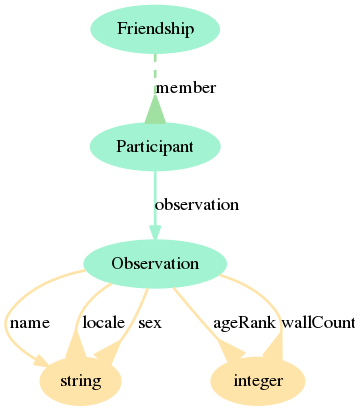
\includegraphics[width=0.5\textwidth]{ontologies/facebook-legacy-AntonioAnzoategui18022013Friendship.ttl/draw}
    \caption{A diagram of the structure involved in the friendship networks
    of the Facebook snapshot. A green edge denotes an OWL existential class restriction; an inverted nip denotes an OWL universal class restriction; a full (non-dashed) edge denotes an OWL functional property axiom. Further information and complete diagrams for each provenance are in the Supporting Information document.}\label{dia}
\end{figure}


\subsection{SPARQL queries}\label{queries}
There are numerous useful and general purpose SPARQL queries to be performed against the database.
Here we write some of the most basic of such queries selected by their potential to be varied.
All queries assume the use the preamble \textttt{PREFIX po: <http://purl.org/socialparticipation/po/>}.
\begin{enumerate}[leftmargin=0cm]
	\item Retrieve the number of participants:\\
            \textttt{SELECT (COUNT(DISTINCT ?author) as ?c) WHERE \{
            ?author a po:Participant . \} }
	\item Retrieve the number of relations, be them interactions or
            friendships:\\
            \textttt{SELECT (COUNT(?interaction) as ?c) WHERE \{\\
                    \h \{ ?interaction a po:Friendship \} UNION \{ ?interaction
                    a po:Interaction \} UNION\\
                    \h \{ ?interaction po:retweetOf
                    ?message \} UNION \{ ?interaction po:replyTo ?message
                    \}\\
                    \h UNION \{ ?interaction po:directedTo ?participant
                    \}\\ \} }
	\item Retrieve all text produced by an specific user:\\
            \textttt{SELECT (CONCAT(?text) as ?texts) WHERE \{\\
                    \h ?activity po:author <user\_uri> . ?activity po:text ?text .\\
    \}}
        \item List 1000 users (URIs and names) with the most friendships and the number of
            friendships in descending order by the number of friendships:\\
            \textttt{SELECT DISTINCT ?participant (COUNT(?friendship)
            as ?c) WHERE \{\\
                \h ?friendship a po:Friendship . ?friendship po:member ?participant . \\
            \} ORDER BY DESC(?c) LIMIT 1000}
        \item Retrieve text messages with the word ``pineapple'' (case insensitive):\\
            \textttt{SELECT ?text WHERE \{ \\
                    \h ?activity po:text ?text . FILTER regex(?text, 'pineapple', 'i')\\
    \}}
\item List participants and respective full names whose name has the substring ``Amanda'':\\
    \textttt{SELECT DISTINCT ?participant ?name WHERE \{\\
    \h ?participant po:observation ?obs . ?obs po:name ?name .\\
    \h FILTER regex(?name, 'Amanda', 'i') \\
    \}}
\item Return all pairs of friends of a participant which are friends themselves:\\
    \textttt{SELECT DISTINCT ?friend1 ?friend2 WHERE \{\\
     \h       ?friendship1 po:member <participant\_uri> .  ?friendship1 po:member ?friend1 .\\
     \h       ?friendship2 po:member <participant\_uri> .  ?friendship2 po:member ?friend2 .\\
     \h       ?friendship3 po:member ?friend1 .  ?friendship3 po:member ?friend2 .\\
    \}}
\item Return all interactions from replies in a snapshot:\\
    \textttt{SELECT ?from ?to WHERE \{\\
          \h  ?message1 po:snapshot <snapshot\_uri> .  ?message2 po:replyTo ?message1 .\\
          \h  ?message1 po:author ?from .  ?message2 po:author ?to .\\
    \}}
\end{enumerate}

\section{License issues}
% Facebook, Twitter, IRC, Gmane, Participa, CD, AA.
The database presented in this article is released under public domain.
Computer scripts are in git repositories and PyPI Python packages, also under public domain.
Although most data is already in open licenses (Twitter, Email, Participabr, Cidade Democrática, and AA data), IRC and Facebook data was collected
and donated by the individuals which yield the data.
This rises the the understanding of the right to study such data as the right to access the self,
in parity with anthropological endaviors~\cite{antphy,antphy2}.
% Of central importance to the obtainment of the data is the concept of
% anthropological physics~\cite{antphy}
\section{Conclusions}
\label{conclusions}
The database presented in this article
constitutes a large database with diverse provenance.
Even so, database should be expanded in upon need or requests from feedback.
All data should be available online in the \url{http://linkedopensocialdata.org}
address in near future to fulfill the purpose of being a common
repertoire in current research.
One should reach the diagrams and tables of the 
Supporting Information document of this article
for further directions
on the available structures and for an overview complement.

% Supporting Information
% diverse provenance, large database, should be expanded, waits feedback
\section*{References}
%
% \bibliographystyle{plainurl}
\bibliography{paper}
%\bibliography{myLastBibfile.bib}
%
\end{document}
